\documentclass[10pt]{beamer}
%\hypersetup{pdfpagemode=FullScreen}
\usepackage[utf8]{inputenc}
\usetheme{Madrid}

% figure configuration
\usepackage{caption}
\captionsetup[figure]{font=scriptsize, justification=centering}

% footnote configuration
\setbeamerfont{footnote}{size=\tiny}

% subfig
\usepackage{subfig}
\captionsetup[subfigure]{font=scriptsize, justification=centering}

% break equation
\usepackage{amsmath}

% outile configuration
\setbeamerfont{section in toc}{size=\large}
\setbeamerfont{subsection in toc}{size=\small}
\setbeamertemplate{section in toc}[sections numbered]
%\setbeamertemplate{subsection in toc}[subsections numbered]

% introduction parameters
\title[Article presentation]{A muscle-reflex model that encodes principles of legged mechanics, produces human walking dynamics and muscle activities}
\subtitle{
	\textbf{Conference}: IEEE Transactions on Neural Systems and Rehabilitation Engineering, June 2010
	\\ \textbf{Authors}: H. Geyer and H. Herr}
\author[J. Charaja and L. Borgonovi]{Jhon Charaja\inst{1} and Luca Borgonovi\inst{1}}
\institute[USP]{
	\inst{1} Universidade de São Paulo, Brasil
}
\date{\today}

% table of contents
\AtBeginSection[]
{
	\begin{frame}
		\frametitle{Outline}
		%\setlength{\parskip}{2ex}
		\tableofcontents[currentsection]
	\end{frame}
}

\AtBeginSubsection[]
{
	\begin{frame}
		\frametitle{Table of contents}
		%\setlength{\parskip}{2ex}
		\tableofcontents[currentsection,currentsubsection]
	\end{frame}
}

% begin document
\begin{document}
	% frame: introduction
	\frame{\titlepage}
	
	\section{Motivation}
	% frame: motivation
	\begin{frame}
		\frametitle{Motivation}
		The bipedal spring-mass model could describes the legged locomotion dynamics\footnotemark[1]
		\begin{columns}
			\column{0.35\textwidth}
			\begin{figure}
				\begin{overprint}
					\onslide<1>\includegraphics[width=.9\textwidth]{images/slip/double_SLIP.pdf}
					\onslide<2>\includegraphics[width=.9\textwidth]{images/slip/double_SLIP_spring_leg.pdf}
					\onslide<3>\includegraphics[width=.9\textwidth]{images/slip/double_SLIP_mass.pdf}
					\onslide<4->\includegraphics[width=.9\textwidth]{images/slip/double_SLIP.pdf}		
				\end{overprint}			
				\caption{Spring-loaded inverted pendulum (SLIP)}
			\end{figure}
			
			\column{0.65\textwidth}
			\begin{itemize}
				\item SLIP model describes the dynamics during walking and running\footnotemark[1] \\[1em]
				\item SLIP model is based on self-stability and compliant leg behavior principles\footnotemark[2] \\[1em]
				\item SLIP model does not present a clear relation with human motor control\footnotemark[2] \\[1em]	
				\item Spinal reflexes can relate sensory information of leg with muscle activation\footnotemark[2]
			\end{itemize}
		\end{columns}
		\footnotetext[1]{H. Geyer (2006).}
		\footnotetext[2]{H. Geyer (2010).}
	\end{frame}
	
	
	\section{Objective}	
	% frame: solution
	\begin{frame}
		\frametitle{Objective}
		\centering
		\LARGE
		\bf
		To develop a neuromuscular human model that encodes the principles of legged locomotion in muscular reflexes
	\end{frame}
	
	\section{Methodology}
	% frame: from SLIP to tree part leg
	\subsection[Methodology]{New model of human lower limb}
	\begin{frame}
		\frametitle{New model of human lower limb}
		\begin{itemize}
			\only<1>{\item Replacing the spring leg with a segmented leg}
			\only<2>{\item Replacing the point of mass with a trunk}
			\only<3,4>{\item Vastus group muscle (VAS) generates knee extension motion
				\item Soleus muscle (SOL) generates ankle plantarflexion motion}
			\only<5>{\item Gastrocnemius muscle (GAS) generates knee flexion and ankle plantarflexion motion
				\item Tibialis anterior muscle (TA) generates ankle dorsiflexion motion}
			\only<6>{\item Gluteus muscle group (GLU) generates negative orientation
				\item Hip flexor muscle group (HFL)  generate positive orientation}	 	 
		\end{itemize}
		\begin{figure}
			\begin{overprint}
				\onslide<1>
				\centering
				\begin{columns}
					\begin{column}{.5\textwidth}
						\centering
						\includegraphics[height=.5\textheight]{images/slip/double_SLIP.pdf}
						\caption{Spring-loaded inverted pendulum (SLIP)}				
					\end{column}
					\begin{column}{.5\textwidth}
						\centering
						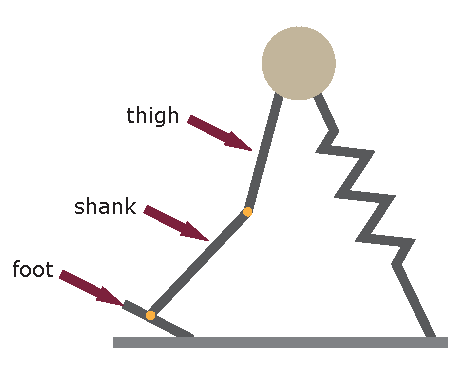
\includegraphics[height=.5\textheight]{images/new_model/left_3leg.pdf} 
						\caption{New model with three segment leg}				
					\end{column}
				\end{columns}
				
				\onslide<2>
				\centering
				\begin{columns}
					\begin{column}{.5\textwidth}
						\centering
						\includegraphics[height=.5\textheight]{images/slip/double_SLIP.pdf}
						\caption{Spring-loaded inverted pendulum (SLIP)}				
					\end{column}
					\begin{column}{.5\textwidth}
						\centering
						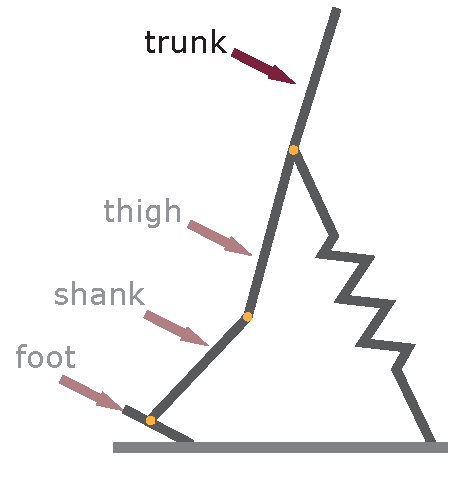
\includegraphics[height=.5\textheight]{images/new_model/left_3leg_trunk.pdf} 
						\caption{New model with three segment leg and a trunk}
					\end{column}	
				\end{columns}	
				
				\onslide<3> 
				\begin{columns}
					\begin{column}{.55\textwidth}
						\centering
						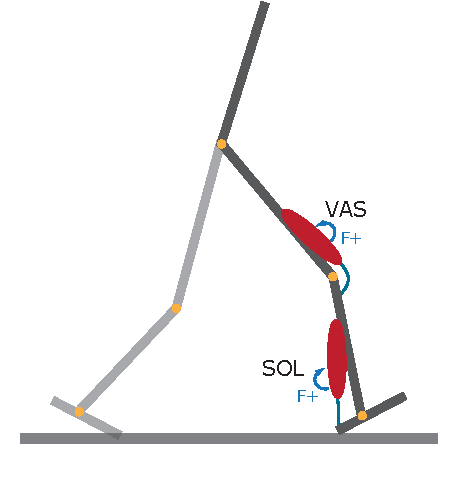
\includegraphics[height=.5\textheight]{images/new_model/stance/muscle_vas_sol.pdf}
						\caption{New bipedal locomotion model with muscles}
					\end{column}
					\begin{column}{.5\textwidth}
						\centering
						\subfloat[Knee extension]{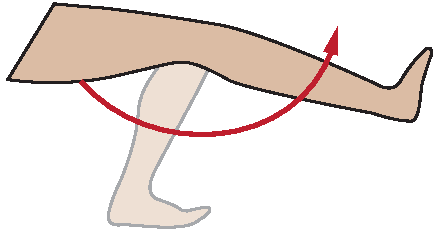
\includegraphics[height=.20\textheight]{images/knee_extension.pdf}} \\
						\subfloat[Ankle dorsiflexion]{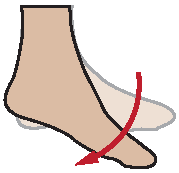
\includegraphics[height=.20\textheight]{images/ankle_planarflexion.pdf}}
					\end{column}  
				\end{columns}
				
				\onslide<4> 
				\begin{columns}
					\begin{column}{.55\textwidth}
						\centering
						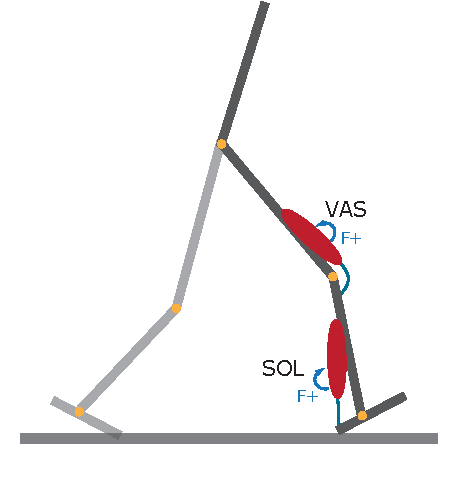
\includegraphics[height=.5\textheight]{images/new_model/stance/muscle_vas_sol.pdf}
						\caption{New bipedal locomotion model with muscles}
					\end{column}
					\begin{column}{.5\textwidth}
						\centering
						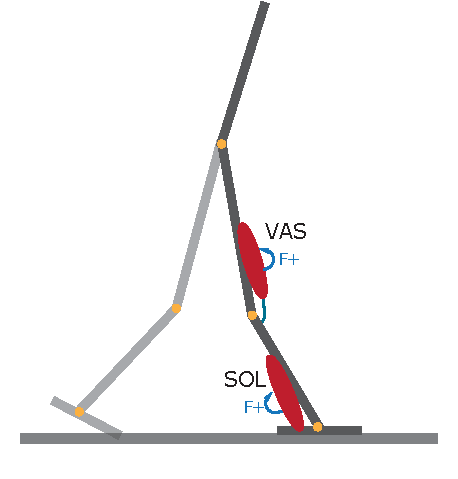
\includegraphics[height=.5\textheight]{images/new_model/stance/muscle_vas_sol_overextension.pdf}
						\caption{overextension case}
					\end{column}  
				\end{columns}
				
				\onslide<5>
				\begin{columns}
					\begin{column}{.5\textwidth}
						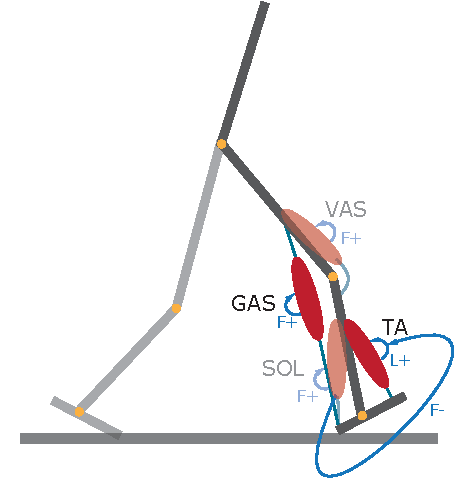
\includegraphics[height=.5\textheight]{images/new_model/stance/muscle_vas_sol_gas_ta.pdf} 
						\caption{New bipedal locomotion model with muscles}
					\end{column}
					\begin{column}{.5\textwidth}
						\begin{itemize}
							\item GAS prevents knee overextension  \\[1em]
							\item GAS contributes to generate compliant behavior \\[1em]
							\item TA prevents ankle overextension
						\end{itemize}
					\end{column}
				\end{columns}
				
				\onslide<6>
				\begin{columns}
					\begin{column}{.5\textwidth}
						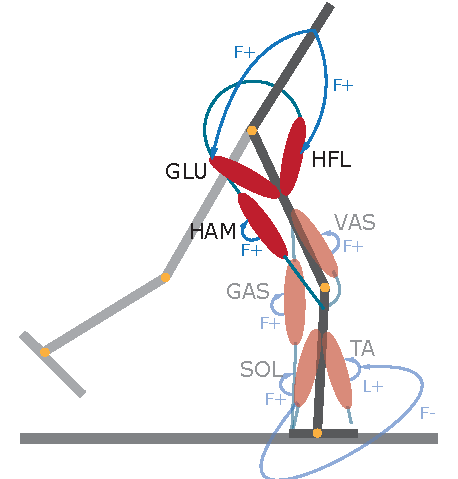
\includegraphics[height=.5\textheight]{images/new_model/stance/muscle_vas_sol_gas_ta_ham_glu_hfl_floor.pdf} 
						\caption{New bipedal locomotion model with muscles}
					\end{column}
					\begin{column}{.5\textwidth}
						\begin{itemize}
							\item GLU and HFL maintain the balance of the trunk  \\ [1em]
							\item Hamstring muscle group (HAM) prevents knee hyperextension
						\end{itemize}
					\end{column}
				\end{columns}	
			\end{overprint}			
		\end{figure}
		
	\end{frame}
	
	\subsection[Methodology]{General equation of muscle stimuli}
	\begin{frame}
		\frametitle{General equation of muscle stimuli}
		\begin{itemize}
			\item Spinal reflexes activate muscles during locomotion
		\end{itemize}
		
		\begin{columns}
			\begin{column}{.5\textwidth}
				\begin{figure}
					\centering
					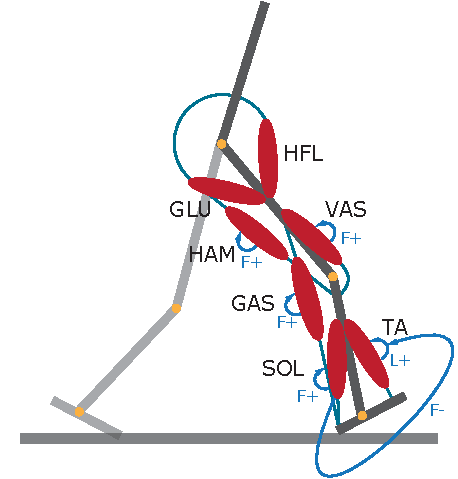
\includegraphics[height=.45\textheight]{images/new_model/stance/muscle_all.pdf}
					\caption{New bipedal locomotion model with muscles}	
				\end{figure}
			\end{column}
			\begin{column}{.5\textwidth}
				\begin{block}{}
					The stimulation of a muscle is given by
					\begin{align*}
						S_{m}(t)&=S_{0,m} + G_{m} F_{m} \delta t_m,  \\
						\delta t_m &= (t-\Delta t_{m}),
					\end{align*}
					where,
					\begin{itemize}
						\item $S_{m}$: stimulation
						\item $S_{0}$: prestimulation
						\item $F_{m}$: force
						\item $G_{m}$: gain
						\item $\Delta t_{m}$: muscle time delay
						\item $\Delta L_m$: muscle stretch
					\end{itemize}
				\end{block}
			\end{column}
		\end{columns}
	\end{frame}
	
	\subsection[Methodology]{Muscle stimuli during the stance phase}
	\begin{frame}
		\frametitle{Stance phase: initial contact}
		\begin{block}{}
			The stimulation of \textbf{VAS} is given by
			\begin{equation*}
				S_{VAS}(t)=S_{0,VAS} + G_{VAS} F_{VAS} (t-\Delta t_{VAS})
			\end{equation*}
		\end{block}
		\begin{block}{}
			The stimulation of \textbf{SOL} is given by
			\begin{equation*}
				S_{SOL}(t)=S_{0,SOL} + G_{SOL} F_{SOL} (t-\Delta t_{SOL})
			\end{equation*}
		\end{block}		
		
		\begin{columns}
			\begin{column}{.5\textwidth}
				\begin{figure}
					\centering
					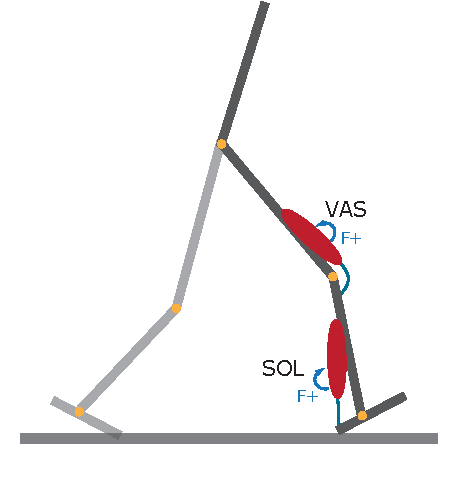
\includegraphics[height=.45\textheight]{images/new_model/stance/muscle_vas_sol.pdf}
					\caption{New bipedal locomotion model with muscles}	
				\end{figure}
			\end{column}
			\begin{column}{.5\textwidth}
				\begin{itemize}
					\item Vastus group muscle (VAS) generates knee extension motion
					\item Soleus muscle (SOL) generates ankle plantarflexion motion
				\end{itemize}
			\end{column}
		\end{columns}
	\end{frame}
	
	\begin{frame}
		\frametitle{Stance phase: initial contact}
		
		\begin{block}{}
			The stimulation of \textbf{GAS} is given by
			\begin{equation*}
				S_{GAS}(t)=S_{0,GAS} + G_{GAS} F_{GAS} (t-\Delta t_{GAS})
			\end{equation*}
		\end{block}
		\begin{block}{}
			The stimulation of \textbf{TA} is given by	
			\begin{equation*}
				S_{TA}(t)=S_{0,TA} + G_{TA} (\Delta L_{TA}) (t-\Delta t_{TA}) - G_{SOL,TA} F_{SOL} (t-\Delta t_{SOL})
			\end{equation*}
		\end{block}		
		
		
		\begin{columns}
			\begin{column}{.5\textwidth}
				\begin{figure}
					\centering
					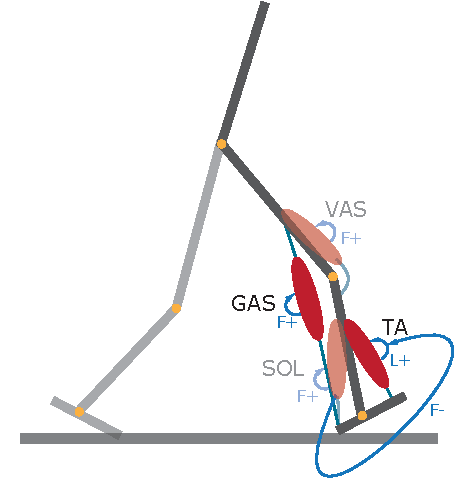
\includegraphics[height=.45\textheight]{images/new_model/stance/muscle_vas_sol_gas_ta.pdf}
					\caption{New bipedal locomotion model with muscles}	
				\end{figure}
			\end{column}
			\begin{column}{.5\textwidth}
				\begin{itemize}
					\item GAS prevents knee overextension 
					\item GAS contributes to generate compliant behavior 
					\item TA prevents ankle overextension
				\end{itemize}
			\end{column}
		\end{columns}
	\end{frame}
	
	
	\begin{frame}
		\frametitle{Stance phase: loading response}
		
		\begin{block}{}
			The stimulation of \textbf{GLU} and \textbf{HFL}  is given by
			\begin{align*}
				S_{GLU}(t) &\sim k_p (\theta-\theta_{ref})_{GLU} + k_d \dot{\theta}_{GLU}, \\
				S_{HFL}(t) &\sim k_p (\theta-\theta_{ref})_{HFL} + k_d \dot{\theta}_{HFL}
			\end{align*}
		\end{block}
		
		\begin{columns}
			\begin{column}{.5\textwidth}
				\begin{figure}
					\centering
					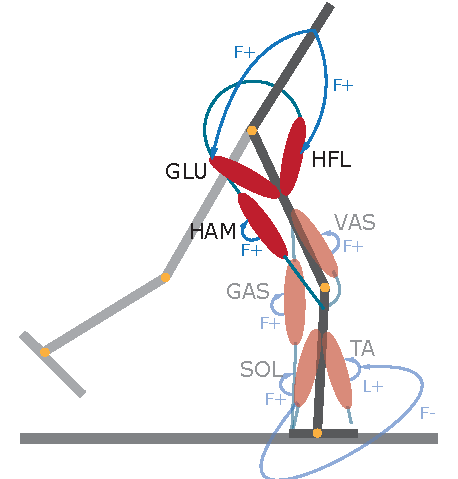
\includegraphics[height=.45\textheight]{images/new_model/stance/muscle_vas_sol_gas_ta_ham_glu_hfl_floor.pdf}
					\caption{New bipedal locomotion model with muscles}	
				\end{figure}
			\end{column}
			\begin{column}{.5\textwidth}
				\begin{block}{}
					The stimulation of \textbf{HAM} is given by	
					\begin{equation*}
						S_{HAM} \sim S_{GLU}
					\end{equation*}
				\end{block}		
				
				\begin{itemize}
					\item GLU generates negative orientation
					\item HAM prevents knee hyperextension
					\item HFL generate positive orientation				
				\end{itemize}
			\end{column}
		\end{columns}
	\end{frame}
	
	
	\subsection[Methodology]{Muscle stimuli during the swing phase}
	\begin{frame}
		\frametitle{Swing phase: pre-swing}
		\begin{block}{}
			The new stimulation of \textbf{VAS} is given by
			\begin{equation*}
				S_{VAS}(t)=S_{0,VAS} + G_{VAS} F_{VAS} (t-\Delta t_{VAS}) - k_{bw}|F_{\textrm{leg}}^{\textrm{ctr}}|
			\end{equation*}
		\end{block}
		
		\begin{columns}
			\begin{column}{.5\textwidth}
				\begin{figure}
					\centering
					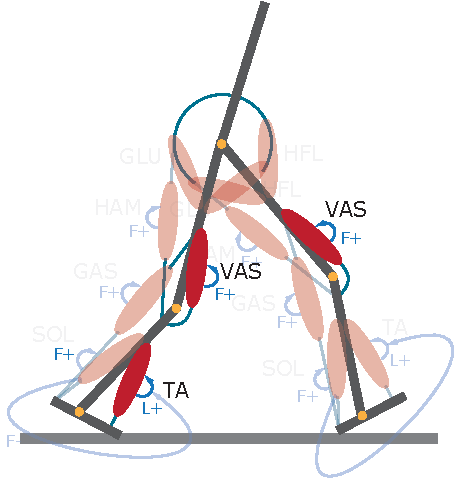
\includegraphics[width=.5\textheight]{images/new_model/swing/muscle_pre_vas.pdf}
				\end{figure}
			\end{column}
			\begin{column}{.5\textwidth}
				where,
				\begin{itemize}
					\item $k_{bw}$: gain proportional to body weight
					\item $F_{\textrm{leg}}^{\textrm{ctr}}$: force applied on contralateral leg
				\end{itemize}
				\begin{exampleblock}{}
					The VAS of swing leg should be inhibit to allow compliance behavior 
				\end{exampleblock}
			\end{column}
		\end{columns}	
	\end{frame}
	
	\begin{frame}
		\frametitle{Swing phase: pre-swing}
		\begin{block}{}
			The new stimulation of \textbf{HFL} and \textbf{GLU} is given by
			\begin{align*}
				S_{HFL}(t)&=  k_p (\theta-\theta_{ref})_{HFL} + k_d \dot{\theta}_{HFL} + \Delta S,  \\
				S_{GLU}(t)&=  k_p (\theta-\theta_{ref})_{GLU} + k_d \dot{\theta}_{GLU} - \Delta S
			\end{align*}
		\end{block}
		
		\begin{columns}
			\begin{column}{.5\textwidth}
				\begin{figure}
					\centering
					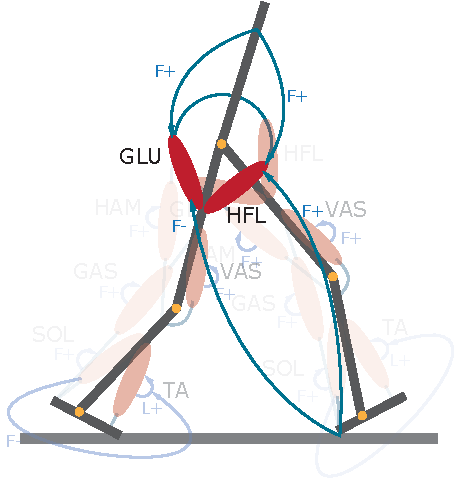
\includegraphics[width=.5\textheight]{images/new_model/swing/muscle_pre_glu.pdf}
				\end{figure}
			\end{column}
			\begin{column}{.5\textwidth}
				where,
				\begin{itemize}
					\item $\Delta S$: constant parameter
				\end{itemize}
				\begin{exampleblock}{}
					The model initiate swing incresing HFL and decresing GLU stimulation
				\end{exampleblock}		
			\end{column}
		\end{columns}	
	\end{frame}
	
	
	\begin{frame}
		\frametitle{Swing phase: initial swing}
		
		\begin{block}{}
			The new stimulation of \textbf{HFL}, \textbf{GLU} and \textbf{HAM} is given by
			\begin{align*}
				S_{HFL}(t)&=  k_p (\theta-\theta_{ref})_{HFL} + G_{HFL}\Delta L_{HFL} - G_{HAM,HFL} \Delta L_{HAM}(t-\Delta t_{HAM}), \\
				S_{GLU}(t)&=  S_{0,GLU} + G_{GLU}F_{GLU}(t-\Delta t_{GLU}), \\
				S_{HAM}(t)&=  S_{0,HAM} + G_{HAM} F_{HAM} (t-\Delta t_{HAM}) 
			\end{align*}
		\end{block}
		
		\begin{columns}
			\begin{column}{.5\textwidth}
				\begin{figure}
					\centering
					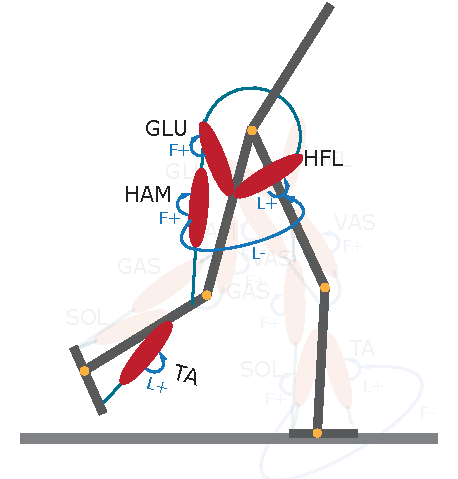
\includegraphics[width=.5\textheight]{images/new_model/swing/muscle_initial.pdf}
				\end{figure}
			\end{column}
			\begin{column}{.5\textwidth}
				\begin{exampleblock}{}
					The new formulation improve gait stability by enforcing swing-leg retraction
				\end{exampleblock}
			\end{column}
		\end{columns}	
	\end{frame}
	
	% luca slides
	\section{Results}
	\subsection[Results]{Walking Gait}
	
	\begin{frame}
		\frametitle{Walking Gait}	
		
		\begin{columns}
			\begin{column}{.5\textwidth}
				\begin{figure}
					\centering
					\includegraphics[height=.45\textheight]{images/graphic_3.pdf}
					\caption{Walking self-organized from dynamic interplay with ground}	
				\end{figure}
			\end{column}
			\begin{column}{.5\textwidth}
				\begin{itemize}
					\item The modeled muscle reflexes include signal transport delays of up to 20 ms
					\item The vertical GRF of the legs in stance shows the M-shape pattern characteristic for walking gaits
				\end{itemize}
			\end{column}
		\end{columns}
	\end{frame}
	
	\subsection[Results]{Steady-State Patterns of Joint Angles and Torques}
	
	\begin{frame}
		\frametitle{Steady-State Patterns of Joint Angles and Torques}
		
		\begin{block}{}
			Maximum cross-correlation coefficients R quantify the agreement between model and human trajectories. $R = 1$ indicates perfect agreement and $R = 0$ indicates no agreement.
		\end{block}	
		
		\begin{columns}
			\begin{column}{.5\textwidth}
				\begin{figure}
					\centering
					\includegraphics[height=.25\textheight]{images/table_quantity_articulation.pdf}
					\caption{Maximum cross-correlation coefficients R for each quantity}	
				\end{figure}
			\end{column}
			\begin{column}{.5\textwidth}
				\begin{itemize}
					\item The performance of the model, in general, is very close to the human movement
					\item The major difference occurs in the knee and hip torques in stance
				\end{itemize}
			\end{column}
		\end{columns}
	\end{frame}
	
	\subsection[Results]{Predicted Motor Output}
	
	\begin{frame}
		\frametitle{Predicted Motor Output}
		
		\begin{columns}
			\begin{column}{.5\textwidth}
				\begin{figure}
					\centering
					\includegraphics[height=.75\textheight]{images/graphic_4.pdf}
					\caption{Maximum cross-correlation coefficients R for each quantity}	
				\end{figure}
			\end{column}
			\begin{column}{.5\textwidth}
				\begin{itemize}
					\item The reflex model produce both walking dynamics and kinematic as predicts known activation patterns
					\item The model can also be evaluated with maximum cross-correlation coefficients R
				\end{itemize}
			\end{column}
		\end{columns}
	\end{frame}
	
	\begin{frame}
		\frametitle{Predicted Motor Output}
		
		\begin{columns}
			\begin{column}{.5\textwidth}
				\begin{figure}
					\centering
					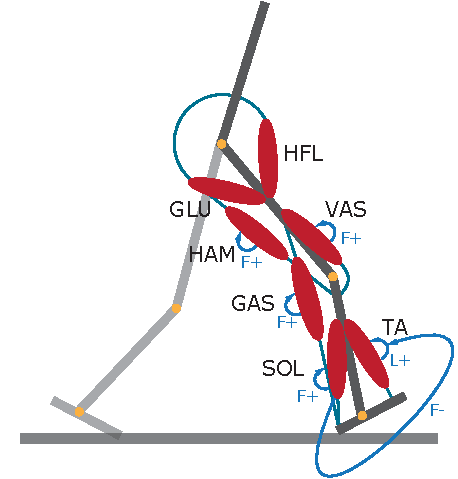
\includegraphics[height=.45\textheight]{images/new_model/stance/muscle_all.pdf}
				\end{figure}
			\end{column}
			\begin{column}{.5\textwidth}
				\begin{figure}
					\centering
					\includegraphics[height=.30\textheight]{images/stance_table.pdf}
					\caption{Maximum cross-correlation coefficients R for each muscle (stance)}	
				\end{figure}
			\end{column}
		\end{columns}
	\end{frame}
	
	\begin{frame}
		\frametitle{Predicted Motor Output}
		
		\begin{columns}
			\begin{column}{.5\textwidth}
				\begin{figure}
					\centering
					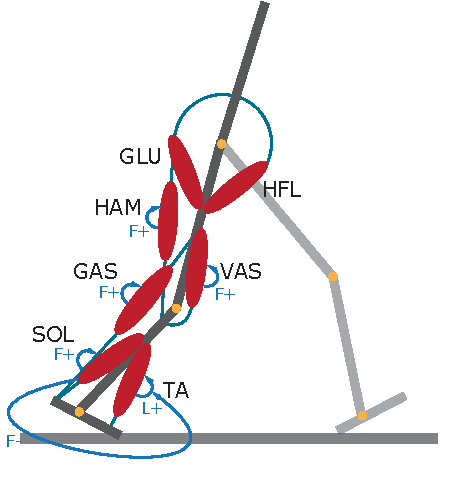
\includegraphics[height=.45\textheight]{images/new_model/swing/muscle_all.pdf}
				\end{figure}
			\end{column}
			\begin{column}{.5\textwidth}
				\begin{figure}
					\centering
					\includegraphics[height=.22\textheight]{images/swing_table.pdf}
					\caption{Maximum cross-correlation coefficients R for each muscle (swing)}	
				\end{figure}
			\end{column}
		\end{columns}
	\end{frame}
	
	\subsection[Results]{Adaptation to Slopes}
	
	\begin{frame}
		\frametitle{Adaptation to Slopes}
		
		The model can adapt to slopes ($ < \pm 4\% $) without parameter interventions.
		
		\begin{figure}
			\centering
			\includegraphics[height=.65\textheight]{images/slope_adaptation.pdf}
			\caption{Slope adaptation}	
		\end{figure}
		
	\end{frame}
	
	\section{Conclusion}	
	% frame: solution
	\begin{frame}
		\frametitle{Conclusion}
		
		\begin{columns}
			\begin{column}{1.0\textwidth}
				\begin{itemize}
					\item Mechanics and motor control cannot be viewed separately in human locomotion
					%\item The principles of legged mechanics were fundamental to simplify the dynamics of walking
					\item After tuning the resulting muscle reflexes that, by combining these principles, human walking dynamics and leg kinematics emerge and the model tolerates ground disturbances and adapts to slopes without parameter interventions
					\item The model predicts some individual muscle activation patterns observed in walking experiments
					\item The interplay between mechanics and motor control is not only important, but could for some muscles dominate human motor output in locomotion
				\end{itemize}
			\end{column}
		\end{columns}
	\end{frame}
	
\end{document}


